% ======================================================================
% 第 14 章：禁闭与渐近自由
% 原著：R. Gupta, "Introduction to Lattice QCD", arXiv:hep-lat/9807028
% 图 10-13；表 6。
% ======================================================================

\chapter{禁闭与渐近自由}

任何理论若要成功描述强相互作用，就必须同时表现出大距离上的禁闭现象与短距离上的渐近自由。格点计算支持这样的假设：对于非阿贝尔规范理论，这两个区域在解析上是相连的，禁闭与渐近自由共存。类似地，表明 QCD 是强相互作用正确理论的一种方式是：在不同能标下（利用实验数据或格点模拟）提取出的耦合常数是唯一的，其含义是它随能标的变化由重整化群给出。$\alpha_s$ 的数据将在第~19 节综述。本节我将讨论这些陈述的含义及其推论。

\section{渐近自由}
\label{sec:asymptotic-freedom}

术语「渐近自由」意味着当探针的动量标度 $\mu \to \infty$ 时，跑动耦合常数 $g \to 0$。这由 $\beta$ 函数刻画：
\begin{equation}
  \mu\frac{\partial g}{\partial\mu}
  = -\beta(g) = -(\beta_0 g^3 + \beta_1 g^5 + \ldots)
  \label{eq:beta-fn}
\end{equation}
其中对非阿贝尔规范群 $\beta(g)$ 为正。在这种情况下，$g = 0$ 是理论的一个紫外稳定不动点，在该点附近可以用标准的微扰展开来分析理论。这一新颖的行为由 't~Hooft、Politzer 以及 Gross 和 Wilczek 所证实，他们证明了微扰 $\beta$ 函数满足式~\eqref{eq:beta-fn} [116]，即对 $N$ 种颜色和 $n_f$ 种活跃味数：
\begin{equation}
  \begin{aligned}
    \beta_0 &= \left(\frac{11N - 2n_f}{3}\right)\!/16\pi^2, \\
    \beta_1 &= \left(\frac{34N^2}{3} - \frac{10N n_f}{3}
               - \frac{n_f(N^2-1)}{N}\right)\!/(16\pi^2)^2.
  \end{aligned}
  \label{eq:beta-coeffs}
\end{equation}
$\beta(g)$ 展开中的这两项领头项在规范与正则化方案下都是不变的。由此容易看出，当 $n_f < 8$ 时 $\beta(g)$ 为正。这一结果对确立 QCD 作为强相互作用理论至关重要，因为它解释了已有的实验数据——这些数据显示，强相互作用的强度随过程中交换动量的增大而减弱。

渐近自由，即式~\eqref{eq:beta-fn}，意味着 QCD 会动力学地产生一个质量标度。为简化标准计算，只保留 $\beta_0$ 项，将式~\eqref{eq:beta-fn} 从动量标度 $\mu_1$ 积分到 $\mu_2$（$\mu_2 > \mu_1$），得到：
\begin{equation}
  \frac{1}{2\beta_0 g^2(\mu_2)} - \frac{1}{2\beta_0 g^2(\mu_1)}
  = \log\frac{\mu_2}{\mu_1},
  \label{eq:integrate}
\end{equation}
即非阿贝尔规范理论的耦合常数随过程的动量标度作对数变化。重写式~\eqref{eq:integrate}：
\begin{equation}
  \begin{aligned}
    \frac{1}{2\beta_0 g^2(\mu)} - \log\mu &= \text{constant} \\
    \implies \exp\left(\frac{1}{2\beta_0 g^2(\mu)}\right)
      &= \frac{\mu}{\Lambda_{QCD}} \\
    \implies \alpha_s(\mu) = \frac{g^2(\mu)}{4\pi}
      &= \frac{1}{8\pi\beta_0\log\frac{\mu}{\Lambda_{QCD}}}
  \end{aligned}
  \label{eq:alpha-s}
\end{equation}
这就引入了 $\Lambda_{QCD}$，即理论中具有质量量纲的不变标度。因此，QCD——一个具有无量纲耦合常数、且在无夸克质量时没有内在质量标度的理论——会动力学地产生一个质量标度。这之所以发生，是因为要确定 $g$，还必须同时指定定义它的动量标度。将上述分析推广到包含式~\eqref{eq:beta-fn} 中的 $\beta_1$ 项，得到：
\begin{equation}
  \Lambda_{QCD} = \lim_{\mu\to\infty}
    \mu \left(\frac{1}{\beta_0 g^2(\mu)}\right)^{\beta_1/2\beta_0^2}
    \exp\left[-\frac{1}{2\beta_0 g^2(\mu)}\right]
    \equiv \mu f_p(g(\mu)) .
  \label{eq:lambda-2loop}
\end{equation}
$\Lambda_{QCD}$ 的这一两圈定义并不唯一；$\Lambda_{QCD}$ 的值依赖于 $g$ 与 $\mu$ 之间的精确关系。然而，一旦在某一个方案中确定了 $\Lambda$ 的值，就可以将其与任何其他微扰方案中的值联系起来。例如，在格点正则化理论中，$\Lambda_{lattice}$ 也由式~\eqref{eq:lambda-2loop} 定义，但其中的 $\mu$ 换成了 $1/a$。于是到一圈近似：
\begin{equation}
  \frac{\Lambda_{QCD}}{\Lambda_{lattice}}
    = \mu a \exp\left[-\left(\frac{1}{2\beta_0 g^2(\mu)}
      - \frac{1}{2\beta_0 g^2(a)}\right)\right].
  \label{eq:lambda-ratio}
\end{equation}
在微扰论中，这两个耦合常数之间的关系为：
\begin{equation}
  g^2(\mu) = g^2(a)\left[1 - \beta_0 g^2(a)\left(\log(\mu a)
    - \log C\right) + O(g^4)\right]
  \label{eq:coupling-rel}
\end{equation}
将式~\eqref{eq:coupling-rel} 代入式~\eqref{eq:lambda-ratio}，可得：
\begin{equation}
  \Lambda_{QCD} = C\, \Lambda_{lattice}
  \label{eq:lambda-C}
\end{equation}
即 $\Lambda_{QCD}$ 与 $\Lambda_{lattice}$ 这两个常数之间仅相差一个乘性常数。要计算 $C$，需要知道耦合常数的有限部分

\begin{table}[htbp]
  \centering
  \begin{tabular}{lccccc}
    \toprule
    $n_f$ & 0 & 1 & 2 & 3 & 4 \\
    \midrule
    $\Lambda_{\overline{MS}}/\Lambda_{latt}$ & 28.8 & 34.0 & 41.1 & 51.0 & 65.5 \\
    $\Lambda_{\overline{MOM}}/\Lambda_{latt}$ & 83.4 & 89.4 & 96.7 & 105.8 & 117.4 \\
    \bottomrule
  \end{tabular}
  \caption{$\Lambda_{\overline{MOM}}$ 和 $\Lambda_{\overline{MS}}$ 与 $\Lambda_{latt}$ 之间的关系，作为活跃味数的函数。$\Lambda_{\overline{MOM}}/\Lambda_{latt}$ 的结果中，$g$ 由三胶子顶点定义，且处于费曼规范下。}
  \label{tab:6}
\end{table}

在格点和连续正则化方案中到一圈的常数重整化 [117,36]。结果列于表~\ref{tab:6}，分别针对 $\Lambda_{\overline{MOM}}$ 和 $\Lambda_{\overline{MS}}$。需要着重指出的是，尽管上述 $\Lambda_{QCD}$ 的定义与估计是用微扰论作出的，但它在本质上是一个非微扰量。

格点模拟中的所有有量纲量都以格距为单位来测量，例如测量的是 $M a$ 而非 $M$。这些无量纲量随 $g$ 的变化为：
\begin{equation}
  M_i a = c_i f_i(g) \equiv c_i \Lambda_i^{\mathrm{non}\text{-}\mathrm{pert}} a .
  \label{eq:scaling-ma}
\end{equation}
其中 $c_i$ 为代表连续值的常数，$f_i$ 是标度函数。当趋近 $g = 0$ 处的不动点时，格点关联长度 $\xi_i \equiv 1/M_i a$ 发散。这一发散是人为造成的——趋于零的是测量单位 $a$，而非 $M_i$。这恰恰是我们希望发生的，以去掉为正则化理论而搭建的脚手架（格点）。非微扰重整化就是在保持某个物理量 $M_i$ 不变的同时，令 $a$ 按 $f_i(g)$ 趋于零来取连续极限。保持不变的特定物理量 $M_i$（弦张力、核子质量等）定义了重整化条件，而 $a$ 与 $g$ 之间的约束就是标度关系。

\begin{itemize}
  \item \textit{标度：}标度假设认为，所有 $f_i(g)$ 都收敛到同一个普适标度函数 $f(g) = \Lambda^{\mathrm{non}\text{-}\mathrm{pert}} a$。此时重整化条件与用于定义它的态无关。对于 $g < g_{scaling}$，每个格点量都由非微扰数 $c_i$ 刻画，所有物理量的无量纲比值都与 $g$ 无关。
  \item \textit{渐近标度：}在 $g = 0$ 处的不动点附近，微扰论适用，所有 $f_i(g) \to f_{pert}(g) \to \Lambda_{QCD} a$。
\end{itemize}

因此，格点模拟可在某一误差容限内，从 $g = 0$ 邻域内的模拟提供连续结果。在此区域内标度成立。对于固定的误差判据，可以通过改进作用量与算符来扩大这一标度窗口，如第~8 节所述。对于在标度窗口之外进行的模拟，必须对 $a = 0$ 作可靠的外推。显然，获得误差上界的一种方法是将测量到的标度函数与 $f_{pert}(g)$ 作比较。好消息是，过去几年的模拟表明，对于格距满足 $5 \lesssim \xi/a < 10$（其中 $\xi/a = 1/(\sqrt{\sigma}\,a)$）的情况，对标度的修正可以降到百分之几的水平。这对应于 $2 \lesssim 1/a \lesssim 4$~GeV。因此，可以在边长约为 $\sim 75 - 150$ 的格点上获得含物理轻夸克的现实结果；而对于许多物理量，如涉及重夸克的那些量，小得多的格点就足够了。格点方法的目标有两个。第一，改进作用量与算符的离散化，把标度区域扩展到更强的耦合；第二，在该区域内多个点处进行模拟，并通过外推到 $a = 0$ 消除剩余误差。

上述讨论的一个推论是：如果 QCD 的所有态在连续极限下都具有零质量，那么 $g = 0$ 将是一个平凡不动点，因为重整化耦合常数 $g_R$ 也将为零。另一方面，人们可以问：QCD 的某些态能否是无质量的，而其余态有质量？值得注意的是，一旦标度行为由式~\eqref{eq:scaling-ma} 固定，我们实际上就能就 QCD 谱的这一方面说出一些内容。事实上，在以下两个假设下，QCD 的纯规范部分将具有质量隙：
\begin{itemize}
  \item 在 $g$ 的任何有限非零值处都不存在零质量态，即在与 $a = 0$ 处连续极限处于同一热力学相的区域中，无量纲量 $M a$ 在任何非零格距 $a$ 处都不为零。
  \item QCD 中只存在一个相关的耦合常数 $g$，与之对应只有一个普适标度函数，例如由式~\eqref{eq:lambda-2loop} 定义。在这种情况下，所有可观测量的标度行为都被固定，在取连续极限时所有质量比都必须保持有限。
\end{itemize}
这两个假设得到了现有数值数据的支持，即在纯规范部分没有无质量态的证据。此外，也没有迹象表明存在分隔已做模拟的区域与 $g = 0$ 的相边界。因此，将格点数据与重整化群标度结合起来，QCD 预言最轻的胶球态是有质量的。

这一预言不因在理论中引入 $n_f$ 种无质量夸克而改变。自发破缺的手征对称性会在谱中产生 $n_f^2 - 1$ 个无质量$\pi$介子。要取手征极限，必须把夸克质量调到零，以定义物理世界。这种调节必须在每个 $a$ 值处进行。因此，不能相对于这些戈德斯通态构造质量比，因为相应的 $c_i(g)$ 已被调到零。

总之，一旦我们验证了标度（微扰的或非微扰的）存在，那么预测 QCD 谱所需的唯一未知量就是常数 $c_i$。渐近自由通过提供 $g \to 0$ 时普适标度行为的解析预言，简化了 QCD。当前数据表明，这些本质上非微扰的系数 $c_i$ 可以利用格点QCD 从 $a \sim 0.1$ 费米处进行的模拟中提取出来。

\section{禁闭}
\label{sec:confinement}

有两种方法可以检验一个理论是否禁闭。其一是证明孤立电荷的自由能是无穷大；其二是证明两个电荷之间的势能随距离增大而增大。第一种检验表明，向系统添加一个孤立的试探电荷需要无穷大的能量；第二种检验则表明，把两个电荷分开到无穷远需要无穷大的能量。我将说明，第一种可由纯规范理论中威尔逊线的期望值 $\langle L\rangle$ 来探测，而第二种可由威尔逊圈的期望值 $\langle W\rangle$ 或关联函数 $\langle L(\tau) L^\dagger(0)\rangle$ 来探测。

\subsection{威尔逊圈}
\label{sec:wilson-loops}

放置在规范场中的外电荷所对应的额外作用量为 $S_J = \int d^4x\, J_\mu^a A_\mu^a$。对于点电荷 $J(x) = \delta^4(x)$，$S_J$ 由规范场沿电荷世界线的路径有序积分给出。于是，对一个 $R \times T$ 矩形威尔逊圈，
\begin{equation}
  W = e^{-S_J} \sim e^{-V(R)T}
  \label{eq:wilson-exp}
\end{equation}
可以把威尔逊圈的期望值理解为：在 $T = 0$ 时刻于 $R/2$ 处产生一个 $qq$ 对，瞬时分开到 $R$ 和 $0$，允许其演化时间 $T$，然后允许其湮灭。在这一过程中，对作用量有贡献的许多项（瞬时产生、湮灭、$\ldots$）中，有一项来自相距为 $R$ 的两个静电荷之间的势能在时间 $T$ 上的积分，即 $V(R)T$。因此，
\begin{equation}
  V(R) = \lim_{T\to\infty} -\frac{1}{T}\log\langle W(R,T)\rangle .
  \label{eq:V-from-W}
\end{equation}
禁闭势最简单的 Ans\"atz 是 Cornell 势：
\begin{equation}
  V(R) = V_0 + \sigma R - \frac{\alpha}{R},
  \label{eq:cornell}
\end{equation}
其中 $\sigma$ 是弦张力。在大距离处 $\sigma R$ 占主导，而在短距离处起作用的则是库仑项 $\alpha/R$。因此，这样的势同时表现出禁闭与渐近自由。对于这样的线性势，大威尔逊圈呈现面积律 $\log\langle W(R,T)\rangle \propto RT$，从而可探测禁闭。Wuppertal 合作组 [118] 对 SU(3) 规范理论的 $V(R)$ 所作的最新计算示于图~\ref{fig:10}。它显示出预期的行为——在大 $R$ 处线性上升，在小 $R$ 处呈库仑行为。

\begin{figure}[htbp]
  \centering
  
\includegraphics[width=0.8\textwidth]{images/fig10.png}
  \caption{淬火近似下的静态 $qq$ 势，由 Wuppertal 合作组 [118] 获得。$\beta = 6.0$、$6.2$、$6.4$ 与 $6.8$ 处的数据已用式~\eqref{eq:sommer} 定义的 $R_0$ 进行标度，并归一化使得 $V(R_0) = 0$。经 $R_0$ 重标度后，各组数据塌缩到同一条曲线上，这是标度存在的证据。大 $R$ 处的线性上升意味着禁闭。}
  \label{fig:10}
\end{figure}

也可以从威尔逊线的关联函数 $\langle L(R) L^\dagger(0)\rangle$ 提取势能，该威尔逊线指向 $T$ 方向、相距为 $R$，定义见第~\ref{sec:wilson-polyakov-line} 节。容易看出，这一关联函数等价于去掉 $T = 0$、$N_T$ 两条边后的威尔逊圈。由于规范链上的周期性边界条件，威尔逊线是闭合的，因此每条威尔逊线单独是规范不变的。这一关联函数度量的是相距为 $R$ 的两个静态试探电荷所对应的作用量。

势能的测量为设定格点计算的标度提供了一种途径。一种方法是使用 $\sigma$。弦张力可以从大 $R$ 处 $V(R)$ 的斜率提取，也可以从 Creutz 比 [120] 的渐近行为提取：
\begin{equation}
  \sigma = \lim_{\substack{T\to\infty\\ R\to\infty}} -\log
    \frac{\langle W(R,T)\rangle \langle W(R+1,T+1)\rangle}
         {\langle W(R+1,T)\rangle \langle W(R,T+1)\rangle}.
  \label{eq:creutz}
\end{equation}
弦张力可以在格点模拟中非常精确地测量，但其物理值要么从 Regge 斜率推断，要么从势模型推断。Regge 现象学给出关系 $M_l^2(l) = l/\alpha' + c$，其中 $M_l$ 是 Regge 轨迹上具有轨道角动量 $l$ 的态的质量。为建立 $\sigma$ 与 $\alpha'$ 之间的关系，采用了两种方法：（1）弦模型给出 $\sigma = 1/2\pi\alpha'$；（ii）势模型给出 $\sigma = 1/8\alpha'$ [123]。$\alpha'$ 的值依赖于夸克质量。例如，由轻强子、$cc$ 和 $bb$ 得到的 $\alpha'$ 分别为 $0.85 \to 0.85/2 \to \approx 0.85/4.5$ GeV$^{-2}$。习惯上选取轻夸克部分的 $\alpha' = 0.85$~GeV$^{-2}$，因为预计它对手势的大距离部分最敏感。将其与弦模型 Ans\"atz $\sigma = 1/2\pi\alpha'$ 相结合，得到 $\sqrt{\sigma} \approx 440$~MeV [124,125]。势模型结果的综述可见 [126]，其中 $\sigma$ 在 $0.18 - 0.22$~GeV$^2$ 范围内变化。在大多数格点计算中使用 $\sqrt{\sigma} = 440$~MeV 这一数值，但人们应当意识到其提取中存在显著的不确定性。

Sommer [127] 提出的一个更好的量是通过两个静电荷之间的力定义的距离标度 $R_0$：
\begin{equation}
  R^2 \left.\frac{\partial V(R)}{\partial R}\right|_{R=R_0} = 1.65
  \label{eq:sommer}
\end{equation}

\begin{figure}[htbp]
  \centering
  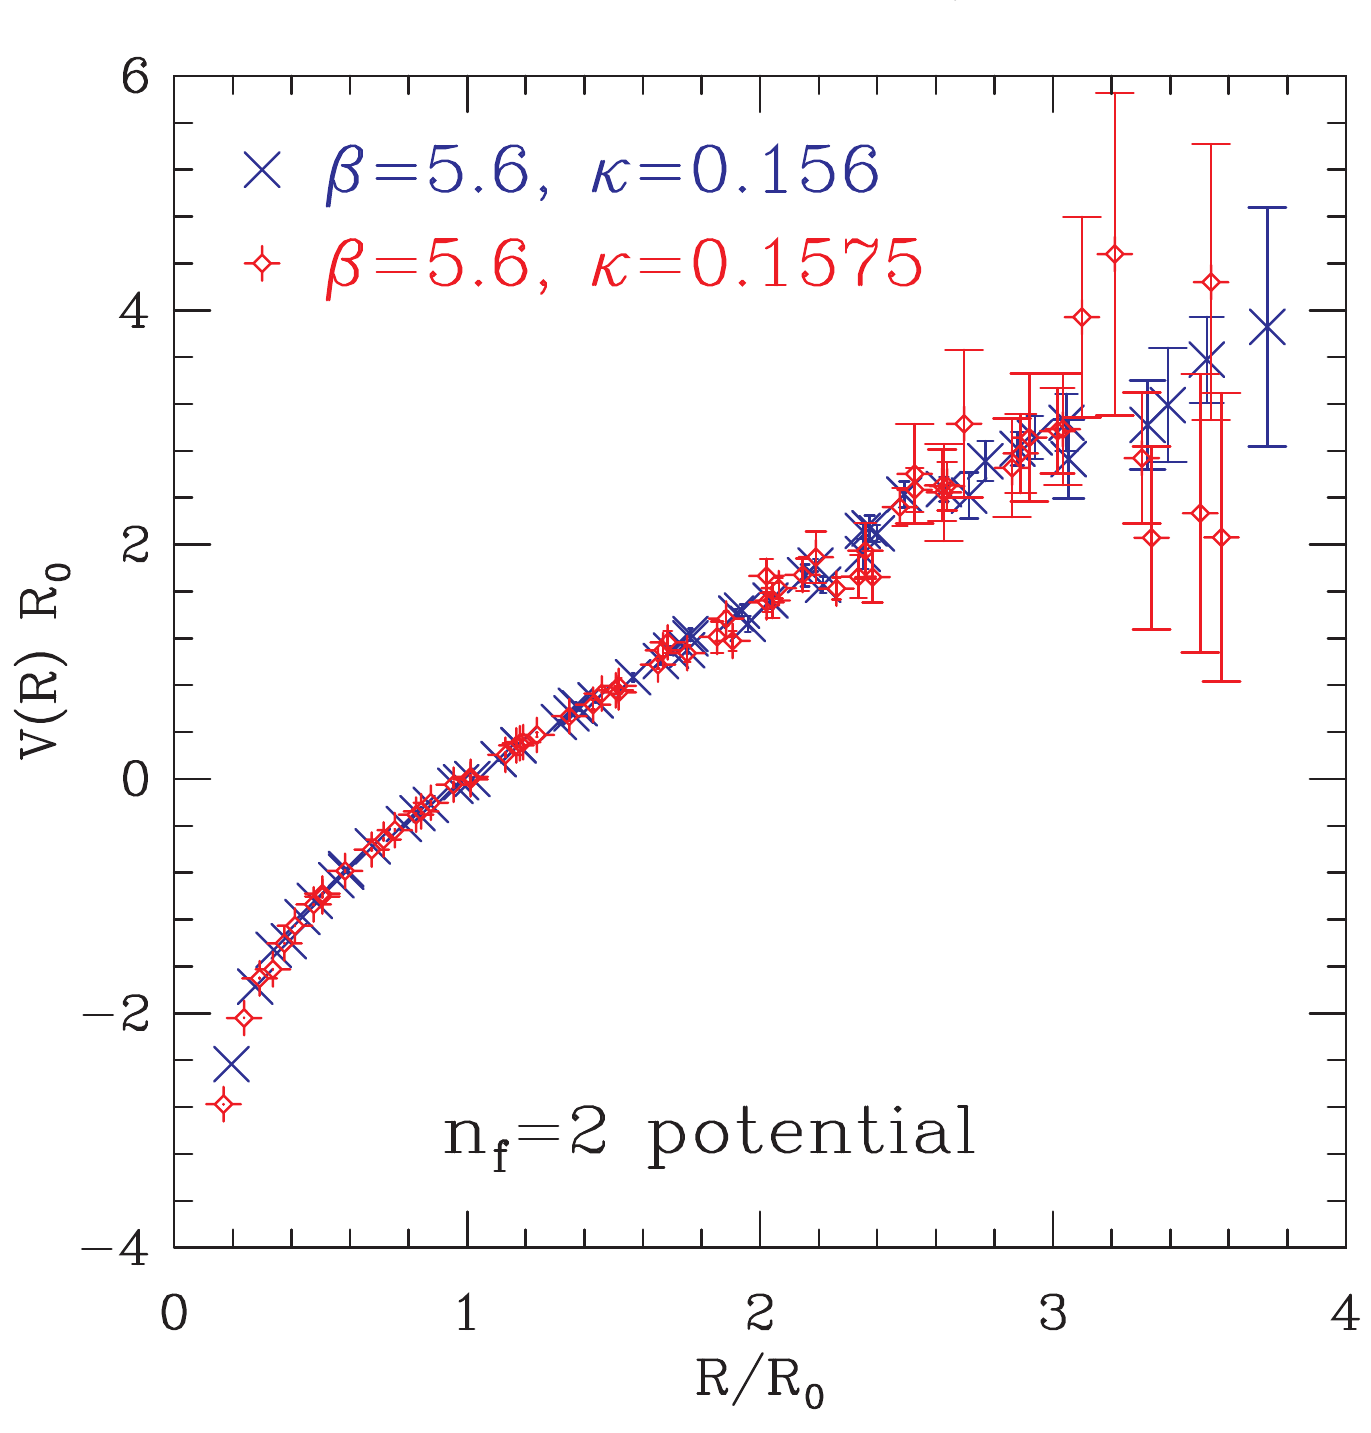
\includegraphics[width=0.8\textwidth]{images/fig11.png}
  \caption{由 Wuppertal 合作组 [119] 获得的含两味动力学费米子的静态 $qq$ 势。在 $\beta = 6.0$、$\kappa = 0.156$ 模拟中动力学费米子质量约为 $\sim 2 m_s$，而在 $\kappa = 0.1575$ 处约为 $\sim m_s$。其余与图~\ref{fig:10} 相同。这些数据比淬火点更低，然而，对于这些动力学费米子质量，尚无大 $R$ 处弦断裂的证据。}
  \label{fig:11}
\end{figure}

在预言粲偶素和 Upsilon 系统能级方面非常成功的 Cornell 势和 Richardson 势给出：
\begin{equation}
  R_0 \approx 0.49~\text{fermi}
  \label{eq:R0}
\end{equation}
使用 $R_0$ 设定标度具有以下优点：（i）其值对唯象势的选择不很敏感；（ii）它定义在一个中间距离处，在该距离上唯象势受到 $cc$ 和 $bb$ 谱的强烈约束；（iii）在这些中间距离上可以高精度地获得 $V(R)$ 的格点测量结果；（iv）这一构造对全 QCD 和淬火 QCD 都成立。来自三个合作组的当前淬火数据状况示于图~\ref{fig:12}。这些数据相互一致，并且在相同的 $\beta$ 范围内，关系 $R_0 = 1.18/\sqrt{\sigma}$ 以非常好的近似成立。（$\sigma$ 由上述 $qq$ 势的大 $R$ 行为提取。）因此，在随后对格点数据的分析中，当使用 $\sigma$ 或 $R_0$ 设定标度时，我将假定这一关系成立。

\begin{figure}[htbp]
  \centering
  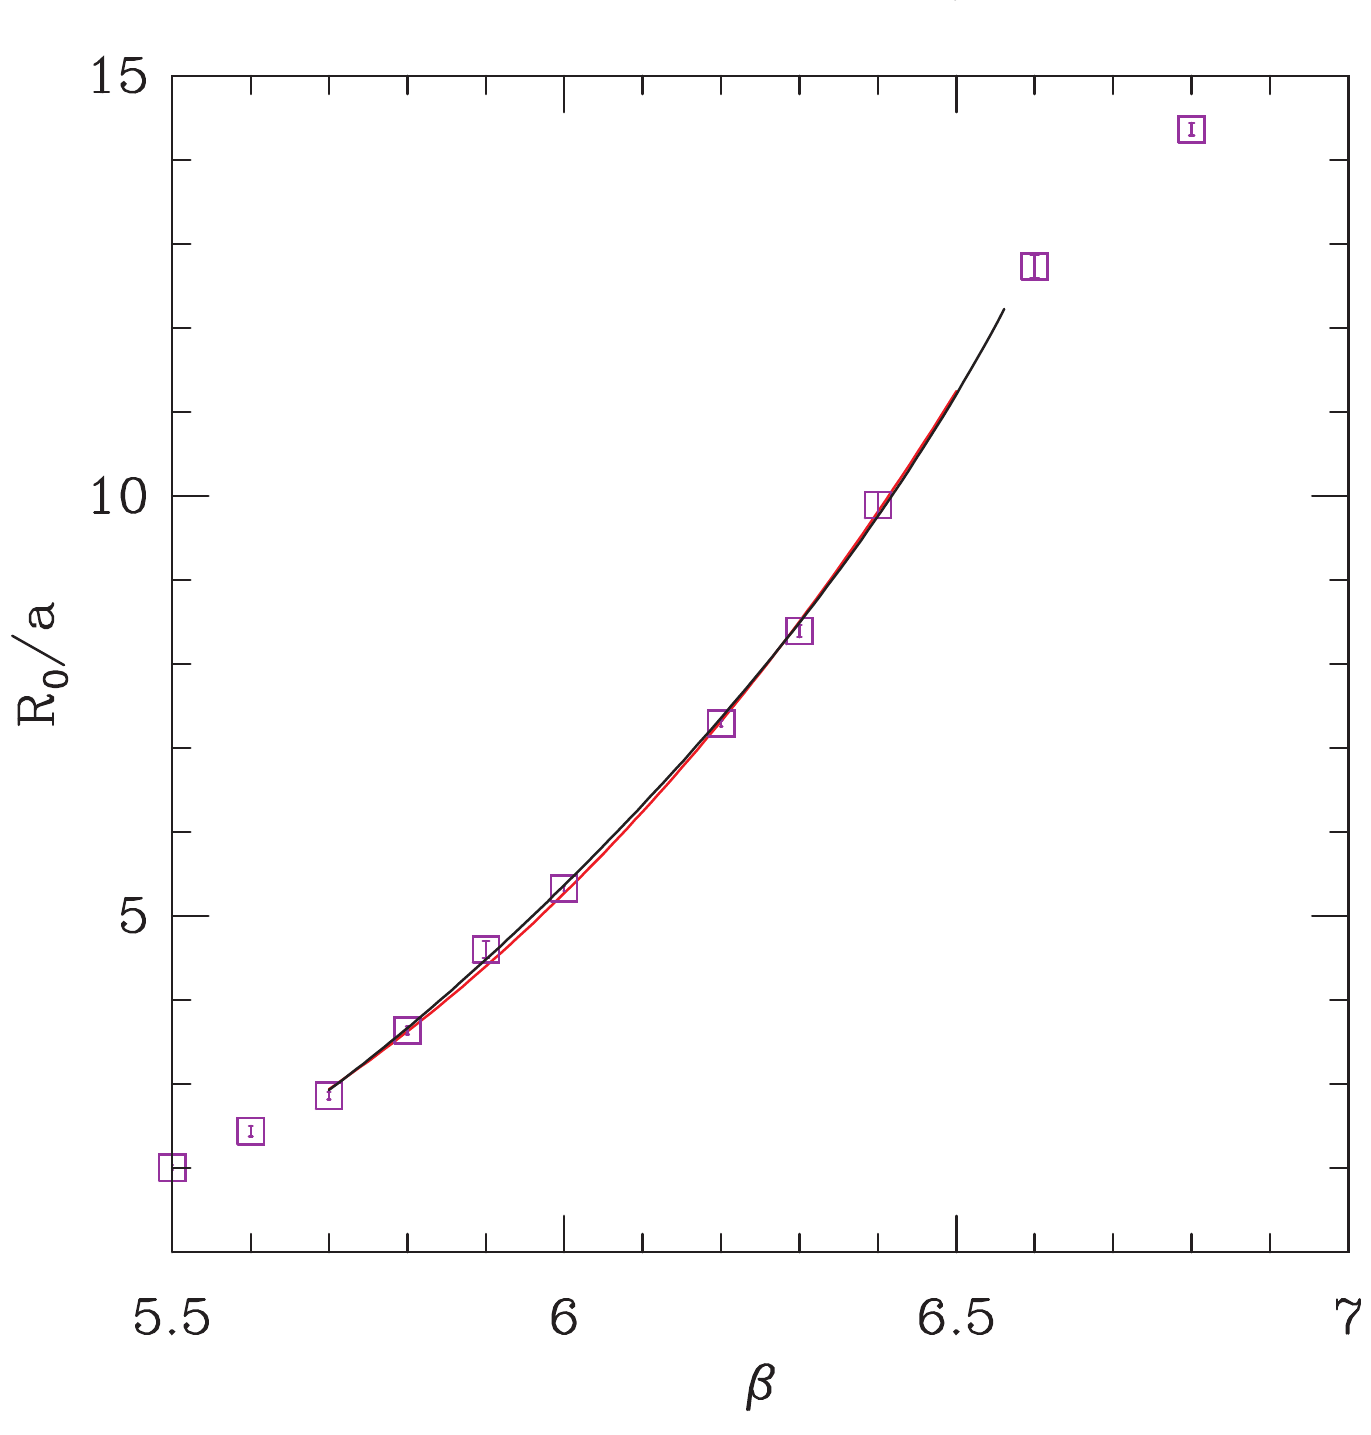
\includegraphics[width=0.8\textwidth]{images/fig12.png}
  \caption{从静态 $qq$ 势提取的标度 $R_0$。紫色数据来自 [118,119,121]，红线是对这些数据的拟合。黑线是 Alpha 合作组 [122] 对数据的拟合：$\log(a/R_0) = -1.6805 - 1.7139(\beta - 6) + 0.8155(\beta - 6.0)^2 - 0.6667(\beta - 6)^3$。}
  \label{fig:12}
\end{figure}

对于全 QCD，线性上升的势能会被屏蔽。当能量大到足以从真空中再激发出一个 $qq$ 对并产生两个介子时，$qq$ 之间的弦就会断裂。这种屏蔽现象可以通过绘制不同动力学费米子质量下的 $V(R)$ 并观察线性上升的变平来检验。发生变平时的 $R/R_0$ 值应随 $m_q$ 减小而减小。最近的一项分析，同样由 Wuppertal 合作组完成，示于图~\ref{fig:11} [119]。数据没有显示出变平——大概是因为该更新中所用的海夸克质量还不够轻，不足以在这些 $R/R_0$ 处引起弦断裂。

\subsection{强耦合展开}
\label{sec:strong-coupling}

对于 $\beta \to 0$，可以用强耦合展开来证明禁闭。我将用两个例子来说明这一技术——弦张力和 $0^{++}$ 胶球质量。

SU($N$) 规范理论的强耦合展开依赖于对链矩阵积分时的以下恒等式：
\begin{align*}
  \int dg &= 1, &
  \int dg\, U_{ij} &= 0, &
  \int dg\, U_{ij}^\dagger &= 0, \\
  \int dg\, U_{ij} U_{kl} &= 0, &
  \int dg\, U_{ij}^\dagger U_{kl}^\dagger &= 0, &
  \int dg\, U_{ij} U_{kl}^\dagger &= \frac{1}{N}\delta_{il}\delta_{jk}
\end{align*}
\begin{equation}
  \int dg\, U_{i_1 j_1}\cdots U_{i_N j_N}
    = \frac{1}{N}\epsilon_{i_1\cdots i_N}\epsilon_{j_1\cdots j_N}.
  \label{eq:group-int}
\end{equation}
要点在于，只有当每条链都以能构成色单态的组合出现时，群积分才会给出非零结果。式~\eqref{eq:group-int} 对恒等式、「介子」和「重子」的链组态说明了这一点。

对小 $\beta$（大 $g$）的方格作用量，威尔逊圈的期望值可以如下展开：
\begin{equation}
  \begin{aligned}
    W_{RT} &= \frac{1}{Z}\int dU\, W_{RT}\,
      e^{(\beta/2N)(W_{11}^{+}+W_{11}^{-})} \\
    &= \frac{1}{Z}\int dU\, W_{RT}\left[1 + \frac{\beta}{2N}\left(W_{11}^{+}
      + W_{11}^{-}\right) + \ldots\right]
  \end{aligned}
  \label{eq:W-expansion}
\end{equation}
其中 $W_{11}^{+}$、$W_{11}^{-}$ 是方格的两个取向，每个圈中颜色指标的求迹是隐含的。考察图~\ref{fig:13}A 可见，积分的第一个非零贡献出现在圈 $W_{RT}$ 被具有正确取向的基本方格铺满时。每个这样的方格从展开中带来一个 $\beta/2N$ 因子，又从积分中带来一个 $1/N$ 因子。（注意 SU(2) 是特殊的，因为圈的两个取向取值相同，即求迹是实的，所以合起来的因子是 $\beta/N^2$。）因此
\begin{equation}
  W_{RT} = \left(\frac{\beta}{2N^2}\right)^{RT}\left(1 + \ldots\right)
  \label{eq:W-area}
\end{equation}
其中领头修正来自把任一给定的铺块替换成一个药盒。现在利用式~\eqref{eq:wilson-exp} 和式~\eqref{eq:cornell} 得到：
\begin{equation}
  \sigma = -\log\frac{\beta}{2N^2} + O(\beta).
  \label{eq:sigma-sc}
\end{equation}
因此，包括 U(1) 在内的所有规范理论在强耦合极限下都禁闭。U(1) 与非阿贝尔规范理论的区别在于，U(1) 规范理论在 $g^2 \sim 1$ 处有一个相变（见第~15 节），而物理理论（电动力学）处于弱耦合区域，该区域与禁闭的强耦合极限在解析上不相连。

作为强耦合展开的第二个应用，考虑 $0^{++}$ 胶球质量的计算。相连的方格-方格关联函数的最小铺块是由四条边组成的矩形管，每条边大小为 $1 \times T$，如图~\ref{fig:13}B 所示。因此
\begin{equation}
  W_{11}(T)W_{11}(0) \sim e^{-M_{0^{++}}T}
    = \left(\frac{\beta}{2N^2}\right)^{4T}\left(1 + \ldots\right),
  \label{eq:glueball}
\end{equation}
以及
\begin{equation}
  M_{0^{++}} = -4\log\frac{\beta}{2N^2} + \ldots .
  \label{eq:Mglueball}
\end{equation}
最低阶结果 $M_{0^{++}}/\sqrt{\sigma} = 4$ 与当今的估计值（见第~18.3 节）非常接近，这一事实纯属偶然。

\begin{figure}[htbp]
  \centering
  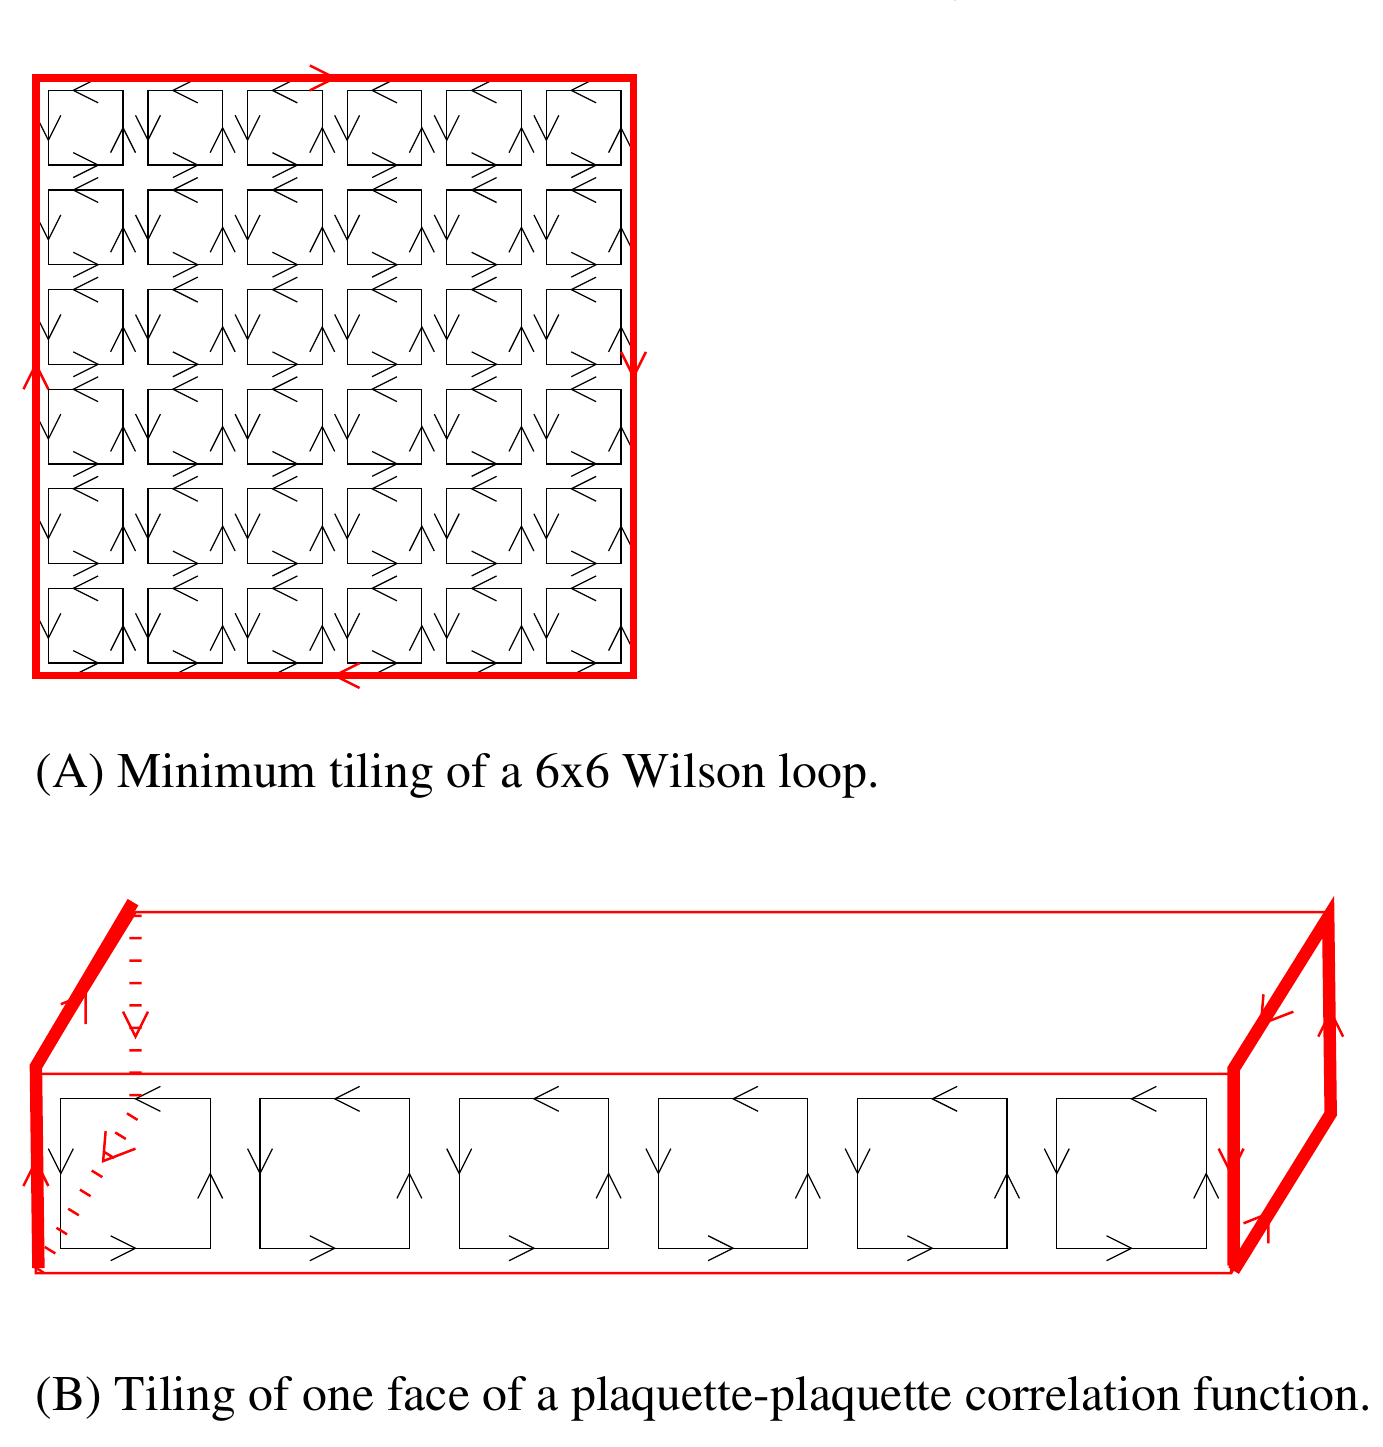
\includegraphics[width=0.8\textwidth]{images/fig13.png}
  \caption{（A）$6 \times 6$ 威尔逊圈和（B）方格-方格关联函数的最小铺块示例。}
  \label{fig:13}
\end{figure}

\textbf{练习：}由 $R \times R$ 威尔逊圈构成的 $0^{++}$ 关联函数的最小铺块是什么？证明式~\eqref{eq:glueball} 与圈的大小无关地成立。

\subsection{威尔逊线/波利亚科夫线}
\label{sec:wilson-polyakov-line}

指向例如时间方向的威尔逊线，由路径有序乘积定义：
\begin{equation}
  \langle L(x,y,z)\rangle = \mathrm{Tr}\, P \prod_{t=1}^{N_T}
    U_4(x,y,z,t)
  \label{eq:polyakov}
\end{equation}
由于规范场的周期性边界条件 $U_4(x,y,z,N_T+1) = U_4(x,y,z,1)$，它是规范不变的。重复以上为威尔逊圈所作的论证，可以发现孤立夸克的自由能由威尔逊线/波利亚科夫线给出：
\begin{equation}
  \langle L\rangle \sim e^{-F_q N_T}.
  \label{eq:free-energy}
\end{equation}
因此，理论中存在孤立电荷的可能性要求 $F_q$ 有限。

除规范不变性之外，SU($N$) 规范理论还具有一个整体 $Z(N)$ 不变性。它包含将给定时间片上的所有链乘以 $Z(N)$ 的同一个元素 $z$，而不改变作用量。在这一变换下 $\langle L\rangle \to z\langle L\rangle$。这样的整体对称性可以被自发破缺。于是我们有两种可能：
\begin{equation}
  \begin{array}{lll}
    \text{Broken:} & \langle L\rangle \neq 0 & \text{Deconfined}\ (F_q\ \text{finite}) \\
    \text{Unbroken:} & \langle L\rangle = 0 & \text{Confined}\ (F_q\ \text{infinite})
  \end{array}
  \label{eq:order-param}
\end{equation}
因此，$\langle L\rangle$ 是一个序参量，用于在纯规范理论中检验禁闭。它也用于探测有限温度相变的位置与级次——$\langle L\rangle$ 的不连续标志着一级相变，而连续变化则意味着二级相变。

Svetitsky 和 Yaffe [128] 论证道，为了确定有限温度相变的级次，相关的有效理论是带 $Z(N)$ 对称性的短程相互作用三维自旋模型（将威尔逊线约化为自旋变量）。然后利用重整化群分析已知的普适类，他们预言 SU(2) 的相变应为二级相变（Ising 类），而 SU($N \geq 3$) 的相变应为一级相变（P\"otts 类）。数值结果与这些预言一致，特别是对 SU(2)，已用统计力学的标准技术确定了临界指数，发现其与三维 Ising 模型一致 [129]。

在存在动力学费米子的情况下，容易看出离散化的 Dirac 作用量在 $Z(N)$ 对称性下不是不变的。因此，对所有 $\beta$ 值都有 $\langle L\rangle \neq 0$，所以 $\langle L\rangle$ 不再是一个序参量。尽管如此，它的变化（不连续或连续）仍被用来寻找有限温度相变的位置及其级次。
